% ============================================================
%  Synchronisation in complete graphs: Cristian, Berkeley, NTP
% ============================================================

\section{Synchronisation in complete graphs}

We now see some algorithms that synchronize physical clocks. We assume that every process can communicate directly with every other process (the communication graph is complete). The algorithms fall into two families:
\begin{itemize}
  \item \textbf{centralized time services}, based on a time server, which can be
  \begin{itemize}
    \item \textit{request-driven}: Cristian's algorithm;
    \item \textit{broadcast-based}: the Berkeley Unix algorithm (Gusella and Zatti, 1989);
  \end{itemize}
  \item \textbf{distributed time services}: the Network Time Protocol (NTP).
\end{itemize}

\subsection{Cristian's algorithm}

Cristian's algorithm\footnote{On the slides the name is written \curlyquotes{Christian}, but the algorithm is due to Flaviu \textit{Cristian} (1989).} is an \textbf{external synchronization} algorithm. It uses a time server $S$ that receives a signal from a UTC source, and every other process synchronizes its clock with $S$.
\begin{itemize}
  \item It works (probabilistically) also in an asynchronous system.
  \item It is based on the measurement of message \textbf{round trip times} (RTTs).
  \item Synchronization is reached only if the RTTs are small with respect to the required accuracy.
\end{itemize}

\begin{framedalgo}[label={alg:cristian}, unbreakable]{Cristian's algorithm}
  \begin{enumerate}
    \item A process $p$ asks the current time to $S$ with a request message $m_r$, and starts measuring the time.
    \item $S$ answers with a message $m_t$ containing $t$, the value of its clock when $m_t$ is sent.
    \item When $p$ receives $m_t$, it measures the round trip time $T_{round}$ and sets its clock to
    \[C_p \gets t + \frac{T_{round}}{2}\]
  \end{enumerate}
\end{framedalgo}

The idea is simple: while the answer travels from $S$ to $p$, the clock of $S$ keeps advancing, so $p$ must add the duration of the trip to $t$. Process $p$ doesn't know this duration, but it knows the duration of the whole round trip, measured with its own clock. Assuming that the request and the answer take the same time, the answer took $T_{round}/2$.

\begin{figure}[H]
  \centering
  \begin{tikzpicture}[xscale=1.3, yscale=1.5]
    \proc{1}{p}{7.2}
    \proc{0}{S}{7.2}
    \node[ev] (a) at (1,1) {};
    \node[ev] (b) at (3,0) {};
    \node[ev] (c) at (5,1) {};
    \draw[msg] (a) -- node[lbl, above right=-1pt] {$m_r$} (b);
    \draw[msg] (b) -- node[lbl, above left=-1pt] {$m_t = t$} (c);
    \node[lbl, below=2pt] at (b) {$S$ reads its clock: $t$};
    \draw[{Latex}-{Latex}] (1,1.35) -- node[above, font=\scriptsize] {$T_{round}$ (measured by $p$)} (5,1.35);
    \node[lbl, above right=2pt, text=RoyalBlue] at (c) {$C_p \gets t + T_{round}/2$};
  \end{tikzpicture}
  \caption{Cristian's algorithm. The answer is assumed to take half of the round trip time.}
  \label{fig:cristian}
\end{figure}

\paragraph{Accuracy.} The two messages don't necessarily take the same time, so the estimate $T_{round}/2$ can be wrong. To bound the error, let $\textit{min}$ be the minimum transmission time of a message, i.e.\ a lower bound on the time a message needs to go from $p$ to $S$ (or vice versa) even when the network is idle. Then the request took at least \textit{min} and the answer took at least \textit{min}, and we have two extreme cases.
\begin{itemize}
  \item \textbf{Case 1}: the real reply time is \textit{greater} than the estimate $RTT/2$. In the worst case the request took exactly \textit{min}, so the reply took $RTT - \textit{min}$. The error of the estimate is
  \[\Delta = \frac{RTT}{2} - (RTT - \textit{min}) = \frac{-RTT + 2\,\textit{min}}{2} = -\frac{RTT}{2} + \textit{min} = -\rbk{\frac{RTT}{2} - \textit{min}}\]
  \item \textbf{Case 2}: the real reply time is \textit{smaller} than the estimate. In the worst case the reply took exactly \textit{min}, and the error is
  \[\Delta = \frac{RTT}{2} - \textit{min}\]
\end{itemize}

\begin{figure}[H]
  \centering
  \begin{subfigure}{0.48\textwidth}
    \centering
    \begin{tikzpicture}[xscale=0.95, yscale=1.3]
      \proc{1}{p}{6.2}
      \proc{0}{S}{6.2}
      \node[ev] (a) at (0.5,1) {};
      \node[ev] (b) at (1.5,0) {};
      \node[ev] (c) at (5.5,1) {};
      \draw[msg] (a) -- node[lbl, left] {$\textit{min}$} (b);
      \draw[msg] (b) -- node[lbl, below right=-2pt] {$RTT - \textit{min}$} (c);
      \draw[{Latex}-{Latex}] (0.5,1.3) -- node[above, font=\scriptsize] {$RTT$} (5.5,1.3);
      \draw[dashed, gray] (3.0,0.9) -- (3.0,1.15) node[above, font=\tiny] {$RTT/2$};
    \end{tikzpicture}
    \caption{Case 1: the reply is slower than estimated.}
  \end{subfigure}
  \hfill
  \begin{subfigure}{0.48\textwidth}
    \centering
    \begin{tikzpicture}[xscale=0.95, yscale=1.3]
      \proc{1}{p}{6.2}
      \proc{0}{S}{6.2}
      \node[ev] (a) at (0.5,1) {};
      \node[ev] (b) at (4.5,0) {};
      \node[ev] (c) at (5.5,1) {};
      \draw[msg] (a) -- node[lbl, below left=-2pt] {$RTT - \textit{min}$} (b);
      \draw[msg] (b) -- node[lbl, right] {$\textit{min}$} (c);
      \draw[{Latex}-{Latex}] (0.5,1.3) -- node[above, font=\scriptsize] {$RTT$} (5.5,1.3);
      \draw[dashed, gray] (3.0,0.9) -- (3.0,1.15) node[above, font=\tiny] {$RTT/2$};
    \end{tikzpicture}
    \caption{Case 2: the reply is faster than estimated.}
  \end{subfigure}
  \caption{The two extreme cases of Cristian's algorithm. In both cases the real reply time differs from $RTT/2$ by at most $RTT/2 - \textit{min}$.}
  \label{fig:cristian-accuracy}
\end{figure}

\begin{framedprop}{Accuracy of Cristian's algorithm}
  The clock of $p$ after the synchronization is accurate within
  \[\pm \rbk{\frac{RTT}{2} - \textit{min}}\]
\end{framedprop}

This explains why synchronization is reached only if the RTTs are small with respect to the required accuracy: the error grows with the RTT. A process can therefore repeat the request several times and keep the answer with the smallest RTT, which gives the best accuracy. This is also why the algorithm works only \textit{probabilistically} in an asynchronous system: there is no bound on the RTT, so there is no guarantee to ever get a small enough one, but in practice it happens with high probability.

\begin{framedex}{}
  Suppose that $p$ measures $RTT = 20$ ms and that the minimum transmission time is $\textit{min} = 4$ ms. Then $p$ sets its clock to $t + 10$ ms, and its clock is accurate within $\pm (10 - 4) = \pm 6$ ms.
\end{framedex}

\begin{framedobs}{}
  If the new value $t + T_{round}/2$ is \textit{smaller} than the current clock of $p$, the clock can't simply be set back: as we saw in \Cref{sec:monotonicity}, it must be slowed down until it reaches the right value.
\end{framedobs}

\paragraph{Discussion.} Cristian's algorithm has some weaknesses:
\begin{itemize}
  \item \textbf{The time server can crash}: it is a single point of failure, and there could be periods in which synchronization is not possible. The solution suggested by Cristian is to use a cluster of synchronized time servers and to ask multiple servers at the same time (a \textit{synchronization group}).
  \item \textbf{The time server can be attacked}: the servers in the group may be arbitrarily faulty or malicious, and a malicious server can make the clocks of all the clients wrong. The solutions are to add redundancy (and use only values on which enough servers agree) and to use authentication, so that clients only trust genuine servers.
\end{itemize}

\subsection{Berkeley's algorithm}

Berkeley's algorithm is an \textbf{internal synchronization} algorithm: there is no UTC source, and the goal is to make all the clocks agree with each other. It has a master-slave structure and it is based on two steps:
\begin{enumerate}
  \item the master gathers the clocks of all the other processes and computes their differences from its own clock;
  \item the master computes a correction for each process and sends it.
\end{enumerate}

\paragraph{Measuring the difference between clocks.} The master process $p_m$ estimates the difference between its clock and the clock of each process $p_i$ as follows:
\begin{enumerate}
  \item $p_m$ sends a message with a timestamp $t_1$ (its local clock value) to each process of the system, $p_m$ included;
  \item when a process $p_i$ receives the message from the master, it sends back a reply with its timestamp $t_2$ (its local clock value);
  \item when the master receives the reply, it reads its local clock ($t_3$) and computes the difference between the clocks.
\end{enumerate}

\begin{figure}[H]
  \centering
  \begin{tikzpicture}[xscale=1.3, yscale=1.5]
    \proc{1}{p_m}{7.2}
    \proc{0}{p_i}{7.2}
    \node[ev] (a) at (1,1) {};
    \node[ev] (b) at (3,0) {};
    \node[ev] (c) at (5,1) {};
    \draw[msg] (a) -- node[lbl, above right=-1pt] {$t_1$} (b);
    \draw[msg] (b) -- node[lbl, above left=-1pt] {$t_2$} (c);
    \node[lbl, above=2pt] at (a) {$t_1$};
    \node[lbl, below=2pt] at (b) {$t_2$};
    \node[lbl, above=2pt] at (c) {$t_3$};
    \draw[dashed, gray] (3,1) -- (3,0.1);
    \node[lbl, above=2pt, gray] at (3,1) {$\frac{t_1+t_3}{2}$};
  \end{tikzpicture}
  \caption{Measuring the difference between the clocks of the master and of $p_i$. As in Cristian's algorithm, the master assumes that $p_i$ read its clock halfway through the round trip.}
  \label{fig:berkeley-measure}
\end{figure}

The slides don't give the formula explicitly, but it is the same idea as Cristian's algorithm: the master assumes that $p_i$ read its clock at the middle of the round trip, when the clock of the master was $\frac{t_1 + t_3}{2}$. Hence, the estimated difference is
\[\Delta p_i = t_2 - \frac{t_1 + t_3}{2}\]
and the estimate is accurate within half of the round trip time $t_3 - t_1$.

\paragraph{The synchronization algorithm.}

\begin{framedalgo}[label={alg:berkeley}, unbreakable]{Berkeley's algorithm}
  \textbf{Master behaviour:}
  \begin{enumerate}
    \item compute the differences $\Delta p_i$ between the master clock and the clock of every process $p_i$ (including the master itself);
    \item compute the average $\textit{avg}$ of all the $\Delta p_i$, \textit{without} considering faulty processes;
    \item compute the correction for each process (including the faulty ones):
    \[\textit{adj}_{p_i} = \textit{avg} - \Delta p_i\]
    and send it to $p_i$.
  \end{enumerate}
  \textbf{Slave behaviour:} each process receives the correction and applies it to its local clock. If the correction is negative, it slows down its clock.
\end{framedalgo}

Here, a process is considered \textbf{faulty} if its clock differs from the clock of the master by more than a given threshold $\gamma$. Faulty processes are excluded from the average, so that a single very wrong clock can't move all the others, but they still receive a correction, so that they get synchronized too.

\begin{framedobs}{}
  The master sends a \textit{correction} (\curlyquotes{move your clock by $+5$}) and not the \textit{new value} of the clock (\curlyquotes{set your clock to 3:00}). This is an important choice: the correction doesn't become obsolete while the message travels, so the delay of the message carrying it doesn't introduce any new error.
\end{framedobs}

\begin{framedex}{Berkeley's algorithm}
  Consider a master $p_m$ and three processes $p_1, p_2, p_3$. When the master's clock reads 3:05, the clocks of the processes read 2:55, 3:00 and 3:25 respectively. The threshold is $\gamma = 10$.

  \textit{Measuring the differences}:
  \begin{align*}
    \Delta p_m &= 3{:}05 - 3{:}05 = 0 \\
    \Delta p_1 &= 2{:}55 - 3{:}05 = -10 \\
    \Delta p_2 &= 3{:}00 - 3{:}05 = -5 \\
    \Delta p_3 &= 3{:}25 - 3{:}05 = +20 \quad \text{(faulty, since } 20 > \gamma\text{)}
  \end{align*}
  \textit{Computing the average} (without $p_3$):
  \[\textit{avg} = \frac{0 - 10 - 5}{3} = -5\]
  \textit{Computing and sending the corrections}:
  \begin{align*}
    \textit{adj}_{p_m} &= \textit{avg} - \Delta p_m = -5 - 0 = -5 \\
    \textit{adj}_{p_1} &= \textit{avg} - \Delta p_1 = -5 - (-10) = +5 \\
    \textit{adj}_{p_2} &= \textit{avg} - \Delta p_2 = -5 - (-5) = 0 \\
    \textit{adj}_{p_3} &= \textit{avg} - \Delta p_3 = -5 - 20 = -25
  \end{align*}
  \textit{Applying the corrections}: all the clocks now read 3:00 (3:05$-$5, 2:55$+$5, 3:00$+$0, 3:25$-$25). The master and $p_3$ have negative corrections, so they slow down their clocks instead of setting them back.
\end{framedex}

\begin{framedobs}{}
  On the slides the difference of $p_3$ is written as $3{:}25 - 3{:}20 = 20$: it is a typo, since the master's clock reads 3:05 (and $3{:}25 - 3{:}20$ would be $5$). The result $+20$ is correct.
\end{framedobs}

\begin{figure}[H]
  \centering
  \begin{tikzpicture}[xscale=0.33, yscale=1.0]
    \draw[-{Latex}] (-1,0) -- (38,0) node[right, font=\scriptsize] {clock value};
    \foreach \x/\l in {5/2:55, 10/3:00, 15/3:05, 20/3:10, 25/3:15, 30/3:20, 35/3:25} {
      \draw (\x,0.1) -- (\x,-0.1) node[below, font=\scriptsize] {\l};
    }
    \draw[ForestGreen!70!black, thick] (10,-0.6) -- (10,2.4);
    \node[ForestGreen!60!black, font=\scriptsize] at (10,2.65) {after: 3:00};
    \node[ev, RoyalBlue] (m) at (15,0.6) {}; \node[font=\scriptsize, right] at (m) {$p_m$ ($-5$)};
    \node[ev, RoyalBlue] (q1) at (5,1.0) {}; \node[font=\scriptsize, left] at (q1) {$p_1$ ($+5$)};
    \node[ev, RoyalBlue] (q2) at (10,1.4) {}; \node[font=\scriptsize, right] at (q2) {$p_2$ ($0$)};
    \node[ev, BrickRed] (q3) at (35,1.8) {}; \node[font=\scriptsize, right, BrickRed] at (q3) {$p_3$ ($-25$, faulty)};
    \draw[msg, gray] (m) -- (10.3,0.6);
    \draw[msg, gray] (q1) -- (9.7,1.0);
    \draw[msg, BrickRed!60] (q3) -- (10.3,1.8);
  \end{tikzpicture}
  \caption{The clocks of the example before (dots) and after (green line) the corrections.}
  \label{fig:berkeley-example}
\end{figure}

\paragraph{Accuracy and fault tolerance.}
\begin{itemize}
  \item The accuracy of the protocol depends on the maximum round trip time: the master does not consider the clock values associated with an RTT greater than a chosen maximum, since their estimate would be too imprecise.
  \item If the master crashes, another master is elected (in an unknown amount of time).
  \item The algorithm is tolerant to arbitrary behaviour, e.g.\ slaves that send wrong values: the master only considers clock values that don't differ from each other by more than a certain threshold (a \textit{fault-tolerant average}).
\end{itemize}

\subsection{Network Time Protocol (NTP)}

Cristian's and Berkeley's algorithms are designed for local networks with a small number of machines. The \textbf{Network Time Protocol} (NTP) is a time service over the Internet, which synchronizes clients with UTC. Its goals are:
\begin{itemize}
  \item \textbf{reliability}, by means of redundant servers and redundant paths between them;
  \item \textbf{scalability}, so that a huge number of clients can synchronize without overloading a few servers.
\end{itemize}

To achieve this, the servers are organized in a hierarchy of levels, called \textbf{strata}:
\begin{itemize}
  \item \textbf{primary servers} (stratum 1) are directly connected to UTC sources (e.g.\ a GPS receiver or an atomic clock);
  \item \textbf{secondary servers} (stratum 2) are synchronized with primary servers;
  \item servers of stratum 3 are synchronized with stratum 2 servers, and so on, down to the lowest level, which consists of the users' computers.
\end{itemize}
The servers form a \textbf{synchronization subnet}. The higher the stratum number, the further a server is from the UTC source, and the less accurate its clock is likely to be, since every level adds the error of one more synchronization.

\begin{figure}[H]
  \centering
  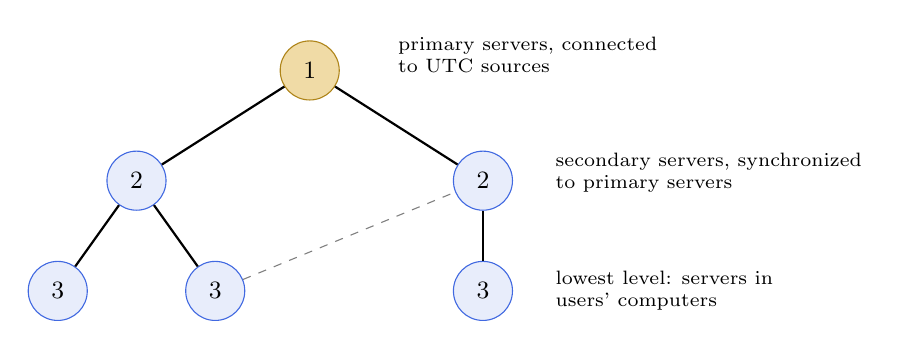
\begin{tikzpicture}[
      srv/.style={circle, draw=RoyalBlue, fill=RoyalBlue!12, minimum size=0.75cm, font=\small},
      level distance=1.4cm,
    ]
    \node[srv, fill=Goldenrod!40, draw=Goldenrod!80!black] (r) at (0,0) {1};
    \node[srv] (a) at (-2.2,-1.4) {2};
    \node[srv] (b) at (2.2,-1.4) {2};
    \node[srv] (c) at (-3.2,-2.8) {3};
    \node[srv] (d) at (-1.2,-2.8) {3};
    \node[srv] (e) at (2.2,-2.8) {3};
    \draw[thick] (r) -- (a); \draw[thick] (r) -- (b);
    \draw[thick] (a) -- (c); \draw[thick] (a) -- (d); \draw[thick] (b) -- (e);
    \draw[dashed, gray] (d) -- (b);
    \node[font=\scriptsize, align=left, anchor=west] at (1.0,0.2) {primary servers, connected\\to UTC sources};
    \node[font=\scriptsize, align=left, anchor=west] at (3.0,-1.3) {secondary servers, synchronized\\to primary servers};
    \node[font=\scriptsize, align=left, anchor=west] at (3.0,-2.8) {lowest level: servers in\\users' computers};
  \end{tikzpicture}
  \caption{The NTP synchronization subnet. Numbers are strata. Redundant links (dashed) allow a server to switch to another one if its parent fails.}
  \label{fig:ntp}
\end{figure}
